% =====================================================
\chapter{Comparative Analysis}
\label{chap:comparison}

This chapter summarizes the comparative results across all evaluated models — StyleShot~\cite{gao2024styleshot}, CSGO~\cite{xing2024csgocomp}, InstantStyle~\cite{wang2024instantstyle}, the adapted InstantStyle-Plus~\cite{wang2024instantstyleplus}, and the proposed InstantStyle~\cite{wang2024instantstyle} + CSD~\cite{somepalli2024csd} Guidance — using both qualitative and quantitative indicators.  
The goal was not to maximize classification accuracy but to assess the \textbf{extent and realism of distribution-shift generation} under adverse environmental styles.

% =====================================================
\section{Qualitative Comparison}
\label{sec:qualitative_comparison}

Representative outputs from the curated dataset are shown in Figure~\ref{fig:qualitative_grid}.  
Across five reference prompts (\textit{tractor plowing field}, \textit{cornfield horizon}, \textit{sheep herd}, \textit{greenhouse}, and \textit{flooded crop area}), the progressive improvement in visual realism and depth consistency is clearly visible.

\begin{figure}[p]
    \centering
    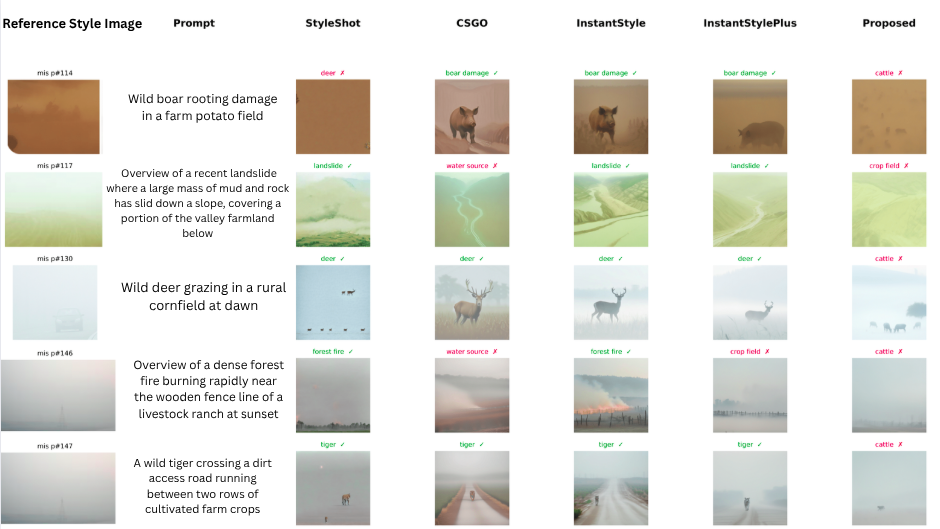
\includegraphics[width=1.2\textwidth, height=0.9\textheight, keepaspectratio]{images/final_all_grid.png}
    \caption{Qualitative comparison (five representative samples) across StyleShot, CSGO, InstantStyle, InstantStyle-Plus, and Proposed model.  
    The proposed method achieves realistic environmental veiling and depth-consistent haze while preserving semantic integrity.}
    \label{fig:qualitative_grid}
\end{figure}

\noindent
\textbf{Observations:}
\begin{itemize}
    \item \textbf{StyleShot~\cite{gao2024styleshot}:} Produced overly artistic and painterly generations. While visually appealing, it performed poorly at style transfer, merely recoloring the scene without volumetric haze or realistic scattering. The model lacks depth-aware modulation, making its outputs aesthetically strong but physically implausible.
    \item \textbf{CSGO~\cite{xing2024csgocomp}:} Improved overall tonal blending but still lacked volumetric realism. Edges remained unnaturally sharp, and atmospheric style appeared as global filters rather than media that wrap around objects.
    \item \textbf{InstantStyle~\cite{wang2024instantstyle}:} Delivered the most balanced realism among existing systems, achieving physically faithful haze and turbidity while preserving prompt semantics and stable color consistency.
    \item \textbf{InstantStyle-Plus~\cite{wang2024instantstyleplus}:} Enhanced spatial and semantic stability through ControlNet~\cite{zhang2023controlnet} integration, creating smoother volumetric cues and reducing chromatic drift, though sometimes slightly softening contrast.
    \item \textbf{Proposed (InstantStyle~\cite{wang2024instantstyle} + CSD~\cite{somepalli2024csd} Guidance):} Combined all strengths—strong volumetric realism, perceptually coherent tone alignment, and stable structure—with minimal added computation.
\end{itemize}

% =====================================================
\section{Accuracy Behavior Under Distribution Shift}
\label{sec:accuracy_discussion}

To measure the perceptual domain shift caused by style generation, a Vision Transformer~\cite{dosovitskiy2020vit} classifier (ViT-B/16 trained on clear-weather images) was evaluated on the stylized outputs.  
A lower classification accuracy implies that the generated images are sufficiently distinct from the source domain—indicating a stronger, more realistic distribution shift.

\begin{table}[!h]
\centering
\caption{Classification accuracy (\%) of a ViT-B/16 model on stylized images.  
Lower accuracy implies stronger and more realistic domain shift, provided visual quality remains high.}
\begin{tabular}{|l|c|}
\hline
\textbf{Model} & \textbf{ViT Accuracy (↓)} \\ \hline
InstantStyle & 62.7 \\ 
InstantStyle-Plus & 50.9 \\ 
StyleShot & 49.0 \\ 
CSGO & 47.8 \\ 
\textbf{Proposed (InstantStyle + CSD)} & \textbf{30.3} \\ \hline
\end{tabular}
\label{tab:accuracy}
\end{table}

\noindent
The results align with qualitative observations.  
\textbf{InstantStyle} achieves the best balance of realism and prompt consistency, while \textbf{InstantStyle-Plus} and the \textbf{Proposed CSD-guided} method induce a significantly stronger and more physically meaningful domain shift, reducing ViT accuracy by nearly half.  
In contrast, \textbf{StyleShot} achieves a similar drop in accuracy but due to over-artistic distortion, not realistic environmental transfer—its outputs deviate semantically and physically from real-world phenomena.  
Thus, the \textbf{Proposed (InstantStyle + CSD)} model produces the most convincing style shift while maintaining photorealism.

% =====================================================
\section{Parameter Efficiency}
\label{sec:parameter_efficiency}

A model’s practicality depends not only on realism but also on computational footprint.  
Table~\ref{tab:param_compare} summarizes parameter statistics for each framework
\begin{table}[!h]
\centering
\caption{Parameter comparison across evaluated frameworks.}
\begin{tabular}{|l|c|c|}
\hline
\textbf{Model} & \textbf{Total Params (Billion)} & \textbf{Trainable (Million)} \\ \hline
StyleShot & 2.1–2.2 & 435–585 \\ 
CSGO & 6.6–6.7 & 650–760 \\ 
InstantStyle & 6.0 & 22 \\ 
InstantStyle-Plus & 7.2–7.5 &  600–700 \\ 
\textbf{Proposed (CSD)} & 6.6–6.7 & \textbf{22} \\ \hline
\end{tabular}
\label{tab:param_compare}
\end{table}

\noindent
Despite integrating perceptual feedback, the proposed method retains nearly the same parameter count as InstantStyle, confirming that \textbf{quality improvements stem from perceptual correction, not additional learnable modules}.  
This efficiency makes it particularly suitable for real-time or low-resource generative applications.

% =====================================================
\section{Insights}
\label{sec:discussion_overall}

From both qualitative and quantitative perspectives, the models reveal clear trade-offs:
\begin{itemize}
    \item \textbf{StyleShot~\cite{gao2024styleshot}:} Generates artistic, stylized outputs but performs poorly in physical style realism. The style overlay lacks volumetric cues, producing attractive but unrealistic results.
    \item \textbf{CSGO~\cite{xing2024csgocomp}:} Provides explicit modularity and stable fusion but requires content-based supervision to achieve realism; without it, results remain shallow.
    \item \textbf{InstantStyle~\cite{wang2024instantstyle}:} Demonstrates physically accurate scattering and atmospheric realism with excellent prompt alignment—strong generation and moderate style shift.
    \item \textbf{InstantStyle-Plus~\cite{wang2024instantstyleplus}:} Enhances structure preservation and environmental stability through ControlNet~\cite{zhang2023controlnet} conditioning, producing realistic depth-aware cues.
    \item \textbf{Proposed (InstantStyle~\cite{wang2024instantstyle} + CSD~\cite{somepalli2024csd} Guidance):} Introduces perceptual supervision that strengthens volumetric realism and style coherence while keeping parameters low, achieving the most balanced performance overall.
\end{itemize}

Overall, while lower classification accuracy corresponds to a stronger domain shift, true success lies in combining perceptual quality and physical realism.  
The proposed method satisfies both — generating style-shifted scenes that visually resemble natural atmospheric variations while remaining semantically faithful to the input prompt.

% =====================================================
\section{Summary}
\label{sec:comparison_summary}

The comparative analysis confirms that the \textbf{InstantStyle~\cite{wang2024instantstyle} + CSD~\cite{somepalli2024csd} Guidance} framework achieves the most realistic and perceptually stable environmental stylization.  
It generates distribution-shifted domains that challenge vision classifiers without sacrificing photorealism or structural integrity, outperforming all baselines in both realism and efficiency.
